\begin{frame}{Conclusiones}
    
    Instrumental en plena medición
    \begin{columns}
        \begin{column}{0.5\textwidth}
            
            \begin{figure}[H]
                \centering
                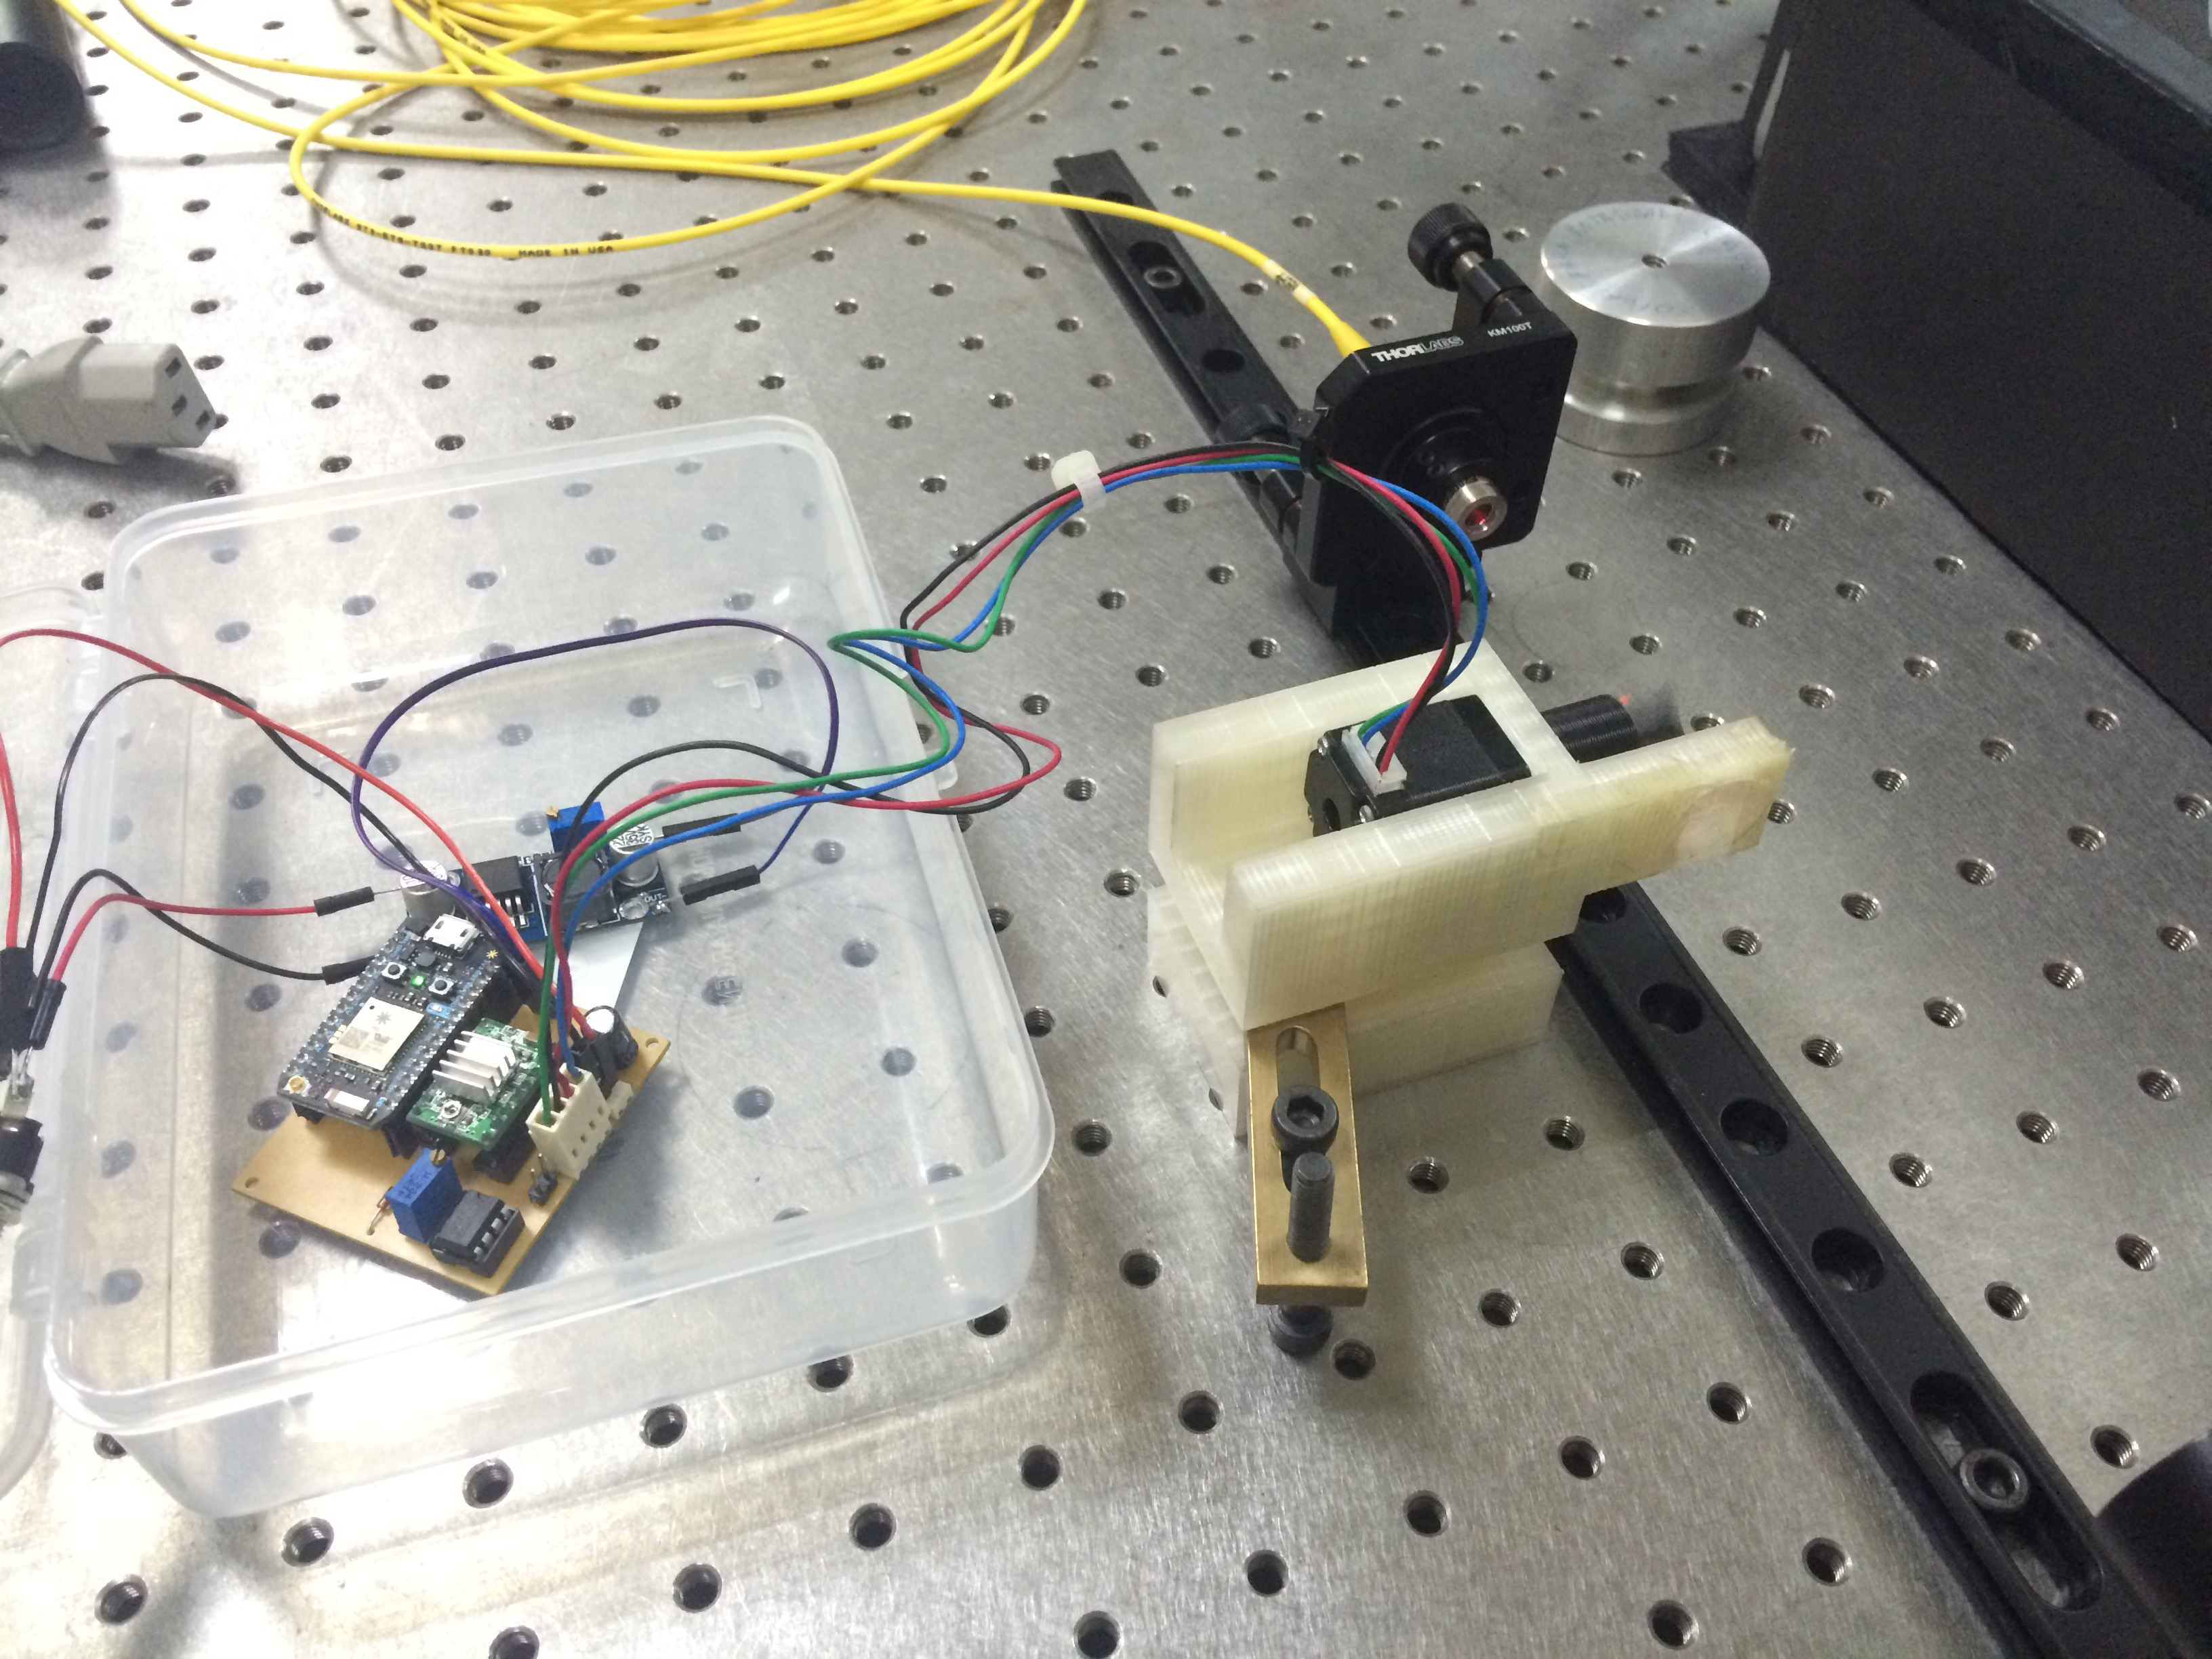
\includegraphics[width=\textwidth]{fig/perfilador/setup_foto}
            \end{figure}
        \end{column}
        
        \begin{column}{0.5\textwidth}
            \begin{figure}[H]
                \centering
                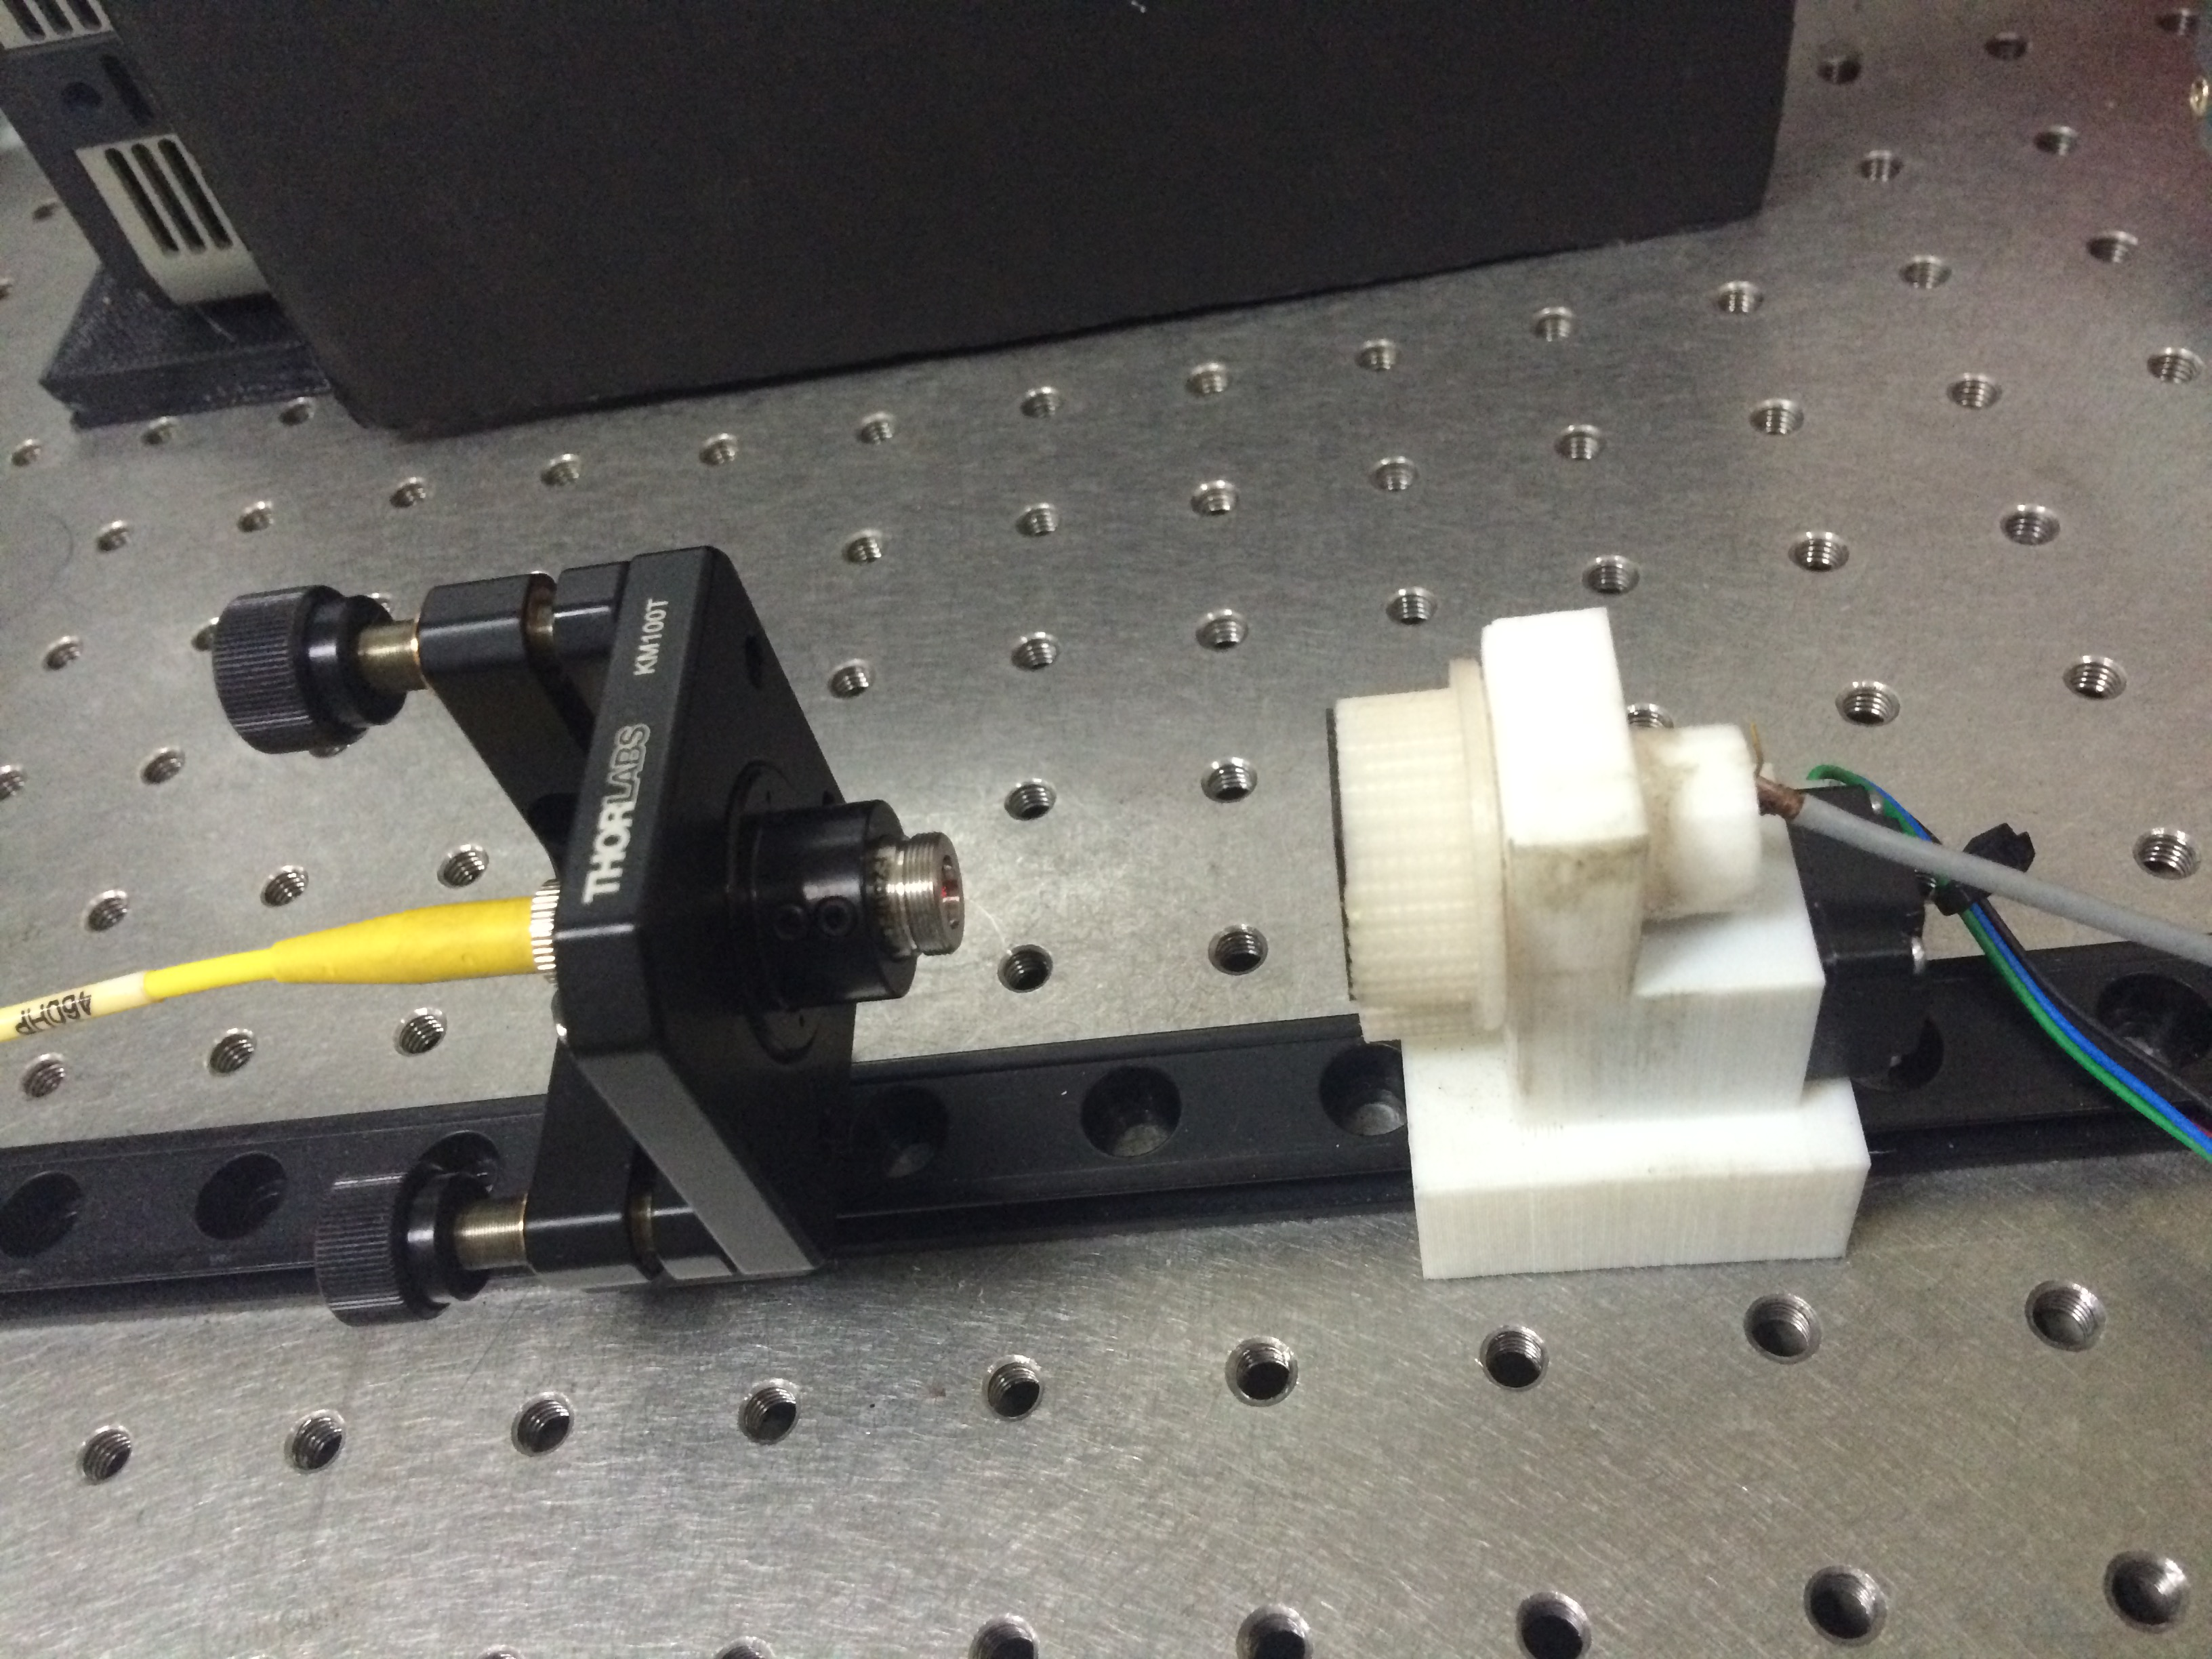
\includegraphics[width=\textwidth]{fig/polarimetro/setup_foto}
            \end{figure}
        \end{column}
    \end{columns}
    %\begin{onlyenv}<1>
    
    
    %Del perfilador
    %    \begin{itemize}
    %        \item El perfilador mide exitosamente el haz, con un error del 5\%, comparable con la medición manual 
    %        \item Se pudo caracterizar el haz a salir de la fibra y en el telescopio correctamente
    %        \item El perfilador fue capaz de medir la divergencia \underline{con solo un set de mediciones}.
    %        \item Para medir la salida del telescopio habrá que diseñar un perfilador más compacto.
    %    \end{itemize}
    %\end{onlyenv}
    
    %\begin{onlyenv}<2>
    %    Del polarimetro
    %    \begin{itemize}
    %        \item La lámina polarizadora utilizada está lejos de ser un polarizador perfecto, pero es funcional a la aplicación
    %        \item Se midió la polarización antes de acoplar en fibra y después de acoplar en fibra y \underline{no se observó cambio de polarización}
    %        \item Esta medición es de importancia fundamental para medir anisotropía de flouroforos en el SPIM
    %    \end{itemize}
    %\end{onlyenv}
\end{frame}
